% gjilguid2e.tex
% V2.0 released 1998 December 18
% V2.1 released 2003 October 7 -- Gregor Hutton, updated the web address for the style files.

%\documentclass[extra,mreferee]{gji}
\documentclass[extra]{gji}
\usepackage{timet}

%Extra packages
\usepackage{graphicx}
\usepackage{amsmath}

\title[Gravity disturbance or gravity anomaly?]
      {Gravity disturbance or gravity anomaly?}
      
\author[Oliveira Jr, Barbosa and Uieda]
{Vanderlei C. Oliveira Jr$^1$\thanks{Sei la, Nacional, Brazil}, Val\'{e}ria C. F. Barbosa$^1$ and Leonardo Uieda$^2$ \\
	$^1$ Department of Geophysics, Observat\'{o}rio Nacional, Rio de Janeiro, Brazil \\
	$^2$ Department of Geology and Geophysics, University of Hawaii, Manoa, USA
}

\date{Received 2018 Month XX; in original form 2018 Month XX}
\pagerange{\pageref{firstpage}--\pageref{lastpage}}
\volume{XXX}
\pubyear{2018}

%\def\LaTeX{L\kern-.36em\raise.3ex\hbox{{\small A}}\kern-.15em
%    T\kern-.1667em\lower.7ex\hbox{E}\kern-.125emX}
%\def\LATeX{L\kern-.36em\raise.3ex\hbox{{\Large A}}\kern-.15em
%    T\kern-.1667em\lower.7ex\hbox{E}\kern-.125emX}
% Authors with AMS fonts and mssymb.tex can comment out the following
% line to get the correct symbol for Geophysical Journal International.
\let\leqslant=\leq

\newtheorem{theorem}{Theorem}[section]

\begin{document}

\label{firstpage}

\maketitle


\begin{summary}
 Gravity anomalies have long been used by geophysicists for the 
 purpose of determining density distributions in subsurface.
 
 However, gravity anomalies 
 
 In this paper, we discuss the fundamental concepts 
 
 URGENTE: \citep{marussi1974}, \citep{torge2012}, section 4.2.1
\end{summary}

\begin{keywords}
 potential fields -- gravity disturbance -- gravity anomaly -- gravity modeling.
\end{keywords}

\section{Introduction}

The resultant of gravitational force and centrifugal force acting 
on a body at rest on the Earth's surface is called 
\textit{gravity vector} and its intensity is called simply 
\textit{gravity} \citep{heiskanen-moritz1967,
hofmann-wellenhof-moritz2005}.
In the case of gravimetry on moving platforms (e.g., airplanes,
helicopters, marine vessels), there are additional
non-gravitational accelerations due to the vehicle motion, 
such as Coriolis acceleration and high-frequency vibrations 
\citep{glennie-etal2000,nabighian-etal2005-grav,baumann-etal2012}.
Geophysicists use gravity for estimating the Earth's 
internal density distribution whereas geodesists use
gravity to estimate the geoid \citep{li2001}.
Hence, geophysicists are usually interested 
in the gravitational component of the observed gravity, 
which is produced by the Earth's internal 
density distribution.
%In applied geophysics, gravity surveys are usually conducted 
%over local or regional areas on the Earth's surface for the purpose of 
%characterizing geological structures located within the
%crust and upper mantle.
%
%Consequently, geophysicists are only interested in the
%particular gravitational component of gravity which 
%is produced by these target geological structures.
The first step of the procedure for isolating this 
gravitational component consists in removing the non-gravitational 
effects due to the vehicle motion and also the time variations 
such as Earth tides, instrumental drift and barometric 
pressure changes, for example.
If these effects are properly removed, the resultant 
gravity data can be considered as the sum of a 
centrifugal component due to the Earth's rotation and
a gravitational component produced by the whole Earth's
internal density distribution.
The isolation of this particular gravitational component 
and its subsequent use for estimating density 
distributions related to geological structures in subsurface 
are the main goals in applied geophysics 
\citep{blakely1996}.

Based on well-established concepts of the literature,
we present a discussion aiming at bringing some
light to the following question: in geophysical applications,
should we use the gravity disturbance or gravity anomaly?
It seems that this theoretical issue has been 
debated within the scientific community from a 
more geodetic than geophysical point of view
\citep{lafehr1991,chapin1996,li2001,fairhead2003,
hackney-featherstone2003,hinze2005}.
Our reasoning suggests that the gravity 
disturbance is more appropriated than gravity anomalies for 
approximating the gravitational effect produced by the Earth's 
internal density distribution.


\section{Normal Earth and normal gravity}

Traditionally, the Earth's gravity field is approximated 
by the gravity field produced by a geocentric and rigid ellipsoid 
of revolution, which has the minor axis $b$ 
coincident with the mean rotating axis of the Earth $Z$, the 
same total mass (including the atmosphere) and also the
same angular velocity of the Earth \citep{heiskanen-moritz1967,
vanicek1987,hofmann-wellenhof-moritz2005,torge2012}.
Another characteristic of this model is that its
limiting surface coincides with a particular equipotential 
of its own gravity field.
Here, we follow \citep{torge2012} and call this model as
\textit{normal Earth}.

Similarly to the gravity vector and gravity, 
the resultant of the virtual 
gravitational and centrifugal forces exerted by the normal
Earth on a body at rest at a point $P$ is called 
\textit{normal gravity vector} and its intensity is called 
simply \textit{normal gravity}.
In geodesy, any model used to represent the normal gravity field
can be arbitrarily defined for the only purpose
of keeping the difference from the actual gravity field as small 
as possible \citep{vanicek1987}.

It is worth noting that, although the normal Earth has the
same total mass (including the atmosphere) of the Earth,
its internal density distribution is unknown.
The search for physically meaningful mass distributions 
that generate a required normal gravity field
has geophysical rather than geodetic motives \citep{marussi1974}.
The only condition imposed on its internal density
distribution is that it produces a gravity field
having a particular equipotential which coincides
with its limiting surface.
For convenience, we denote any density distribution 
satisfying this condition as a \textit{normal density distribution}.

The normal Earth gives rise to the \textit{geodetic coordinate system}
\citep{heiskanen-moritz1967, soler1976, torge2012, bouman_etal2013}.
In this coordinate system, the position of a point $P$
is defined by the \textit{geometric height} $h$, 
\textit{geodetic latitude}
$\varphi$ and \textit{longitude} $\lambda$ (Figure \ref{fig:fig1}).
Geodetic coordinates $(h, \varphi, \lambda)$ can be easily 
converted into geocentric Cartesian coordinates $(X, Y, Z)$
(Figure \ref{fig:fig1}).
The plane containing the point $P$, the axis $Z$ and
the origin $O$ of this \textit{geocentric Cartesian coordinate system}
is called meridian plane (gray plane in Figure \ref{fig:fig1}).
At a given point $(h, \varphi, \lambda)$, there are three 
unit vectors (Figure \ref{fig:fig1}) given by \citep{soler1976}:
\begin{equation}
\begin{split}
\hat{\mitbf{u}} &= 
\begin{bmatrix}
\cos\varphi \, \cos\lambda \\
\cos\varphi \, \sin\lambda \\
\sin\varphi
\end{bmatrix} \\
\hat{\mitbf{v}} &= 
\begin{bmatrix}
-\sin\varphi \, \cos\lambda \\
-\sin\varphi \, \sin\lambda \\
\cos\varphi
\end{bmatrix} \\
\hat{\mitbf{w}} &= 
\begin{bmatrix}
-\sin\lambda \\
\cos\lambda \\
0
\end{bmatrix}
\end{split} \: ,
\label{eq:unit-vectors}
\end{equation}
Notice that these unit vectors are mutually orthogonal and
that the normal gravity vector $\mitbf{\gamma}_{P}$ at a point $P$
is opposite to the unit vector $\hat{\mitbf{u}}_{P}$ at $P$.


\section{Gravity disturbance}

It is worth noting that, by definition, 
the centrifugal component of the normal gravity field is
equal to the centrifugal component of the Earth's gravity
field if they are evaluated at the same point.
Then, the differences between the gravity vector
(corrected from non-gravitational effects) 
and the normal gravity vector, at the same point, represents a purely 
gravitational and consequently harmonic disturbing field.
This gravitational disturbance 
is caused by contrasts between the actual internal 
density distribution of the Earth and the internal density 
distribution of the normal Earth.
In applied geophysics, these density differences are generally 
called \textit{anomalous masses} (e.g., \citeauthor{hammer1945}, 
\citeyear{hammer1945}; \citeauthor{lafehr1965}, \citeyear{lafehr1965}),
\textit{density anomalies} (e.g., \citeauthor{forsberg1984}, \citeyear{forsberg1984})
or \textit{gravity sources} (e.g., \citeauthor{blakely1996}, 
\citeyear{blakely1996}). Here, we opted for using the last term.

The difference between the observed gravity and the
normal gravity, at the same point, is called \textit{gravity disturbance}
\citep{heiskanen-moritz1967, hofmann-wellenhof-moritz2005}.
Notice that the gravity disturbance is not equivalent to the
magnitude of the difference between the gravity vector
and the normal gravity vector at the same point 
\citep{barthelmes2013, sanso_sideris2013}.
As properly pointed out by \citet{hackney-featherstone2003},
the gravity disturbance is a very-well established quantity in geodesy,
but appears to be less well known in geophysics.

The gravity anomaly is the commonly used quantity in applied 
geophysics. It is defined as the difference
between the gravity on the geoid and the normal gravity on the ellipsoid,
both at the same geodetic latitude and longitude.
Notice that, by definition, the gravity anomaly depends on 
longitude and latitude only and is not a function in space 
\citep{barthelmes2013}.
Different gravity anomalies can be calculated, depending on the
corrections applied to them \citep{blakely1996, hofmann-wellenhof-moritz2005}.
These corrections are usually called gravity reductions.
For example, the Free-air anomaly is an approximation of the
gravity disturbance whereas the Bouguer anomaly
is an approximation of the terrain corrected gravity disturbance.
The last one is commonly used by geophysicists as the
gravitational effect produced by the gravity sources.
Although this approximation is valid for most practical applications,
it is important to bear in mind not only the terminology 
changes, but also the conceptual assumptions.

There was a certain lack of comprehension regarding the
geophysical meaning of gravity anomalies until the
mid 90's.
As properly pointed out by \citet{chapin1996} at that time, 
``although the corrections which bring about a Bouguer 
gravity anomaly are well established, the reasons for doing
them are not well understood. One cause of this common 
misunderstanding is that the subject has been poorly presented in
many of the basic texts".
In his seminal book, \citet{blakely1996} brought some light
on the geophysical meaning of gravity anomalies from the 
perspective of applied geophysics. \citet{blakely1996} correctly
defined gravity sources as density contrasts between the actual
internal density distribution of the Earth and the internal density
distribution of the normal Earth.
However, he did not stress that, by removing the normal gravity 
evaluated on the ellipsoid from the gravity measured 
on the Earth's surface, the remaining disturbing field will reflect 
not only the effect produced by the gravity sources, but also a
small combination of gravitational and centrifugal effects.
This additional, non-harmonic and undesired effect is 
simply due to the calculation of the normal gravity at a point
other than that were the gravity is measured.


\section{Mathematical description of the gravity disturbance in a local coordinate system}

In a local- or regional-gravity study, 
geophysicists commonly use a topocentric Cartesian coordinate system
with origin at a point $P$ and axes $x$, $y$ and $z$ defined
by the unit vectors $\hat{\mitbf{v}}_{P}$,
$\hat{\mitbf{w}}_{P}$ and $-\hat{\mitbf{u}}_{P}$ 
(equation \ref{eq:unit-vectors}), respectively
(Figures \ref{fig:fig1} and \ref{fig:fig2}).
In this coordinate system, the observed gravity vector
$\mitbf{g}_{i}$, at a point $(x_{i}, y_{i}, z_{i})$, 
$i = 1, ..., N$, can be represented by
\begin{equation}
\mitbf{g}_{i} = \mitbf{\gamma}_{i} + \Delta \mitbf{g}_{i} \: ,
\label{eq:gravity-vector}
\end{equation}
where $\mitbf{\gamma}_{i}$ and $\Delta \mitbf{g}_{i}$
are, respectively, the normal gravity vector and a
disturbing gravitational attraction produced by the anomalous 
masses at the point $(x_{i}, y_{i}, z_{i})$.

For each point $(x_{i}, y_{i}, z_{i})$ in the topocentric
Cartesian coordinate system (Figure \ref{fig:fig2}b), there is
a corresponding point $(h_{i}, \varphi_{i}, \lambda_{i})$
in the geodetic coordinate system (Figure \ref{fig:fig1}).
Here, we opted for omitting the equations to convert a point
$(x_{i}, y_{i}, z_{i})$ into a point $(h_{i}, \varphi_{i}, \lambda_{i})$
and vice versa. These equations, however, may be easily
found in the literature \citep[e.g.,][]{heiskanen-moritz1967, soler1976, torge2012, bouman_etal2013}.

By definition, the gravity disturbance $\delta g_{i}$,
at the point $(x_{i}, y_{i}, z_{i})$, is given by 
\citep{heiskanen-moritz1967, hofmann-wellenhof-moritz2005}:
\begin{equation}
\delta g_{i} =  g_{i} - \gamma_{i} \: ,
\label{eq:gravity-disturbance}
\end{equation}
where $g_{i} = \| \mitbf{g}_{i} \|$ and 
$\gamma_{i} = \| \mitbf{\gamma}_{i} \|$ are,
respectively, the observed gravity and the normal gravity at the
point $(x_{i}, y_{i}, z_{i})$.
Fortunately, the condition 
$\gamma_{i} \gg \| \Delta \mathbf{g}_{i} \|$ 
is met at all points located above or on the Earth's surface.
By combining this condition and the definition of observed gravity vector
(equation \ref{eq:gravity-vector}), we can approximate the observed gravity
$g_{i}$ by a first order Taylor's expansion as follows 
\citep{sanso_sideris2013}:
\begin{equation}
g_{i} \approx \gamma_{i} + 
\hat{\mitbf{\gamma}}_{i}^{\top} \Delta \mitbf{g}_{i} \: ,
\label{eq:gobs-approx}
\end{equation}
where $^{\top}$ denotes transposition,
$\hat{\mitbf{\gamma}}_{i} = -\hat{\mitbf{u}}_{i}$ is a unit 
vector with the same direction as the normal gravity vector 
$\mitbf{\gamma}_{i}$ at the point $(x_{i}, y_{i}, z_{i})$, in the
topocentric Cartesian coordinate system (Figure \ref{fig:fig2}b), and
$\hat{\mitbf{u}}_{i}$ is the unit vector $\hat{\mitbf{u}}$ 
(equation \ref{eq:unit-vectors}) evaluated at the corresponding 
point $(h_{i}, \varphi_{i}, \lambda_{i})$ in the 
geodetic coordinate system (Figure \ref{fig:fig1}).

This approximation, which is known in geodesy \citep[e.g.,][]{sanso_sideris2013},
is largely used in applied geophysics for representing
total-field anomalies \citep[e.g.,][]{blakely1996}.
Notice that, in local- or regional-gravity studies, the unit
vector $\hat{\mitbf{\gamma}}_{i}$ (equation \ref{eq:gobs-approx}) 
may be considered constant throughout the study area and 
parallel to the $z$ axis of the topocentric Cartesian coordinate 
system (Figure \ref{fig:fig2}b).
Consequently, by using the approximation defined in equation 
\ref{eq:gobs-approx}, the gravity disturbance 
(equation \ref{eq:gravity-disturbance}) can be rewritten as 
follows 
\begin{equation}
\delta g_{i} \approx \hat{\mitbf{\gamma}}_{P}^{\top} \Delta \mitbf{g}_{i} \: ,
\label{eq:gravity-disturbance-approx}
\end{equation}
where $\hat{\mitbf{\gamma}}_{P}$ represents the unit vector with
the same direction as the normal gravity vector $\mitbf{\gamma}_{P}$
at the origin $P$ of the topocentric Cartesian coordinate system
(Figure \ref{fig:fig2}).
This equation shows that the gravity disturbance $\delta g_{i}$ (equation \ref{eq:gravity-disturbance}) is different from the magnitude
of the disturbing gravitational attraction $\Delta \mitbf{g}_{i}$
produced by the gravity sources. Rather, it represents the 
component of the $\Delta \mitbf{g}_{i}$ on the direction of the normal
gravity vector. In the topocentric Cartesian coordinate system,
the gravity disturbance $\delta g_{i}$ (equation \ref{eq:gravity-disturbance-approx})
can be defined as the vertical component of the gravitational attraction exerted by
the gravity sources at the point $(x_{i}, y_{i}, z_{i})$.
As a consequence, the gravity disturbance produced by
a homogeneous gravity source with density contrast $\Delta\rho$
(in $kg / m^{3}$) can be represented by the following harmonic function:
\begin{equation}
d_{i} = k_{g} \, G \, \Delta\rho \, \partial_{z} \phi_{i} \: ,
\label{eq:gz-local}
\end{equation}
where $G$ is the Newtonian constant of gravitation
(in $m^{3} / (kg \, s^{2})$),
$k_{g} = 10^{5}$ is a constant factor
transforming from $m/s^{2}$ to milligal (mGal),
and $\partial_{z} \phi_{i}$ is a harmonic function representing the first 
derivative, evaluated at the observation point $(x_{i},y_{i},z_{i})$, 
$i = 1, ..., N$, of the function 
\begin{equation}
\phi(x,y,z) = \int\int\limits_{v}\int \frac{1}{\sqrt{(x - x^{\prime})^{2} + 
(y - y^{\prime})^{2} + (z - z^{\prime})^{2}}} \: dv
\label{eq:phi}
\end{equation}
with respect to the variable $z$. The 
integral is conducted over the coordinates $x^{\prime}$, $y^{\prime}$ 
and $z^{\prime}$ within the volume $v$ of the gravity source.
This equation can be easily generalized for the case
of multiple gravity sources.

Practically all the literature about gravity modeling
use the quantity $d_{i}$ (equation \ref{eq:gz-local})
to represent the gravity anomaly produced by 
gravity sources \citep[e.g.,][]{blakely1996}. 
Consequently, almost all the geophysicists use the gravity
anomaly as an approximation of the gravity disturbance
produced by the gravity sources. Notice that $d_{i}$ 
(equation \ref{eq:gz-local}) does not depend on the
geoidal surface. Rather, it depends on the relative position 
of the observation points $(x_{i}, y_{i}, z_{i})$ with respect to
the gravity sources in a topocentric Cartesian coordinate
system (Figure \ref{fig:fig2}b).


\section{Conclusions}

We debate the conceptual differences between the gravity
disturbance and the gravity anomaly.
Our reasoning suggest that the gravity disturbance is the
more appropriated quantity for representing the gravity
effect produced by the gravity sources.
In summary, we point out that:

\begin{enumerate}
%\renewcommand{\theenumi}{(\arabic{enumi})}
\renewcommand{\theenumii}{\alph{enumii}}

\item Almost all interpretation techniques assume, implicitly or
directly, that the gravity data is harmonic (e.g., 
upward/downward continuation, 
data processing with equivalent layer,
conversions between gravity and magnetic data,
computation of vertical derivatives via Fourier and Hilbert
transforms). As a consequence, they implicitly or directly assume that
the gravity data approximates the gravitational disturbance.

\item Almost all forward modeling techniques compute
the vertical component of the gravitational attraction 
exerted by the geological bodies at the observation points.
Notice that the gravity anomaly requires the computation of gravity
on the Geoid, which is generally within the topographic masses.
Hence, almost all geophysicists implicitly compute 
the gravity disturbance.

\item The gravity anomaly is defined as the difference between 
the gravity on the Geoid and the normal gravity on the reference 
ellipsoid, both at the same geodetic latitude and longitude.
Consequently, the gravity anomaly is a function of
the geodetic latitude and longitude only and cannot
be calculated at arbitrary heights. On the other hand,
the gravity disturbance can be computed at arbitrary points
outside the sources.

\end{enumerate}

The principal theoretical implication of this study is that
is that, although the gravity anomaly may be used as a good approximation of
the gravity effect produced by the sources for most practical applications,
the more appropriated quantity for gravity modeling is the
gravity disturbance. We stress that, more important than the 
the terminology changes, the geophysicist must bear in mind the 
conceptual assumptions used in gravity modeling.


\begin{acknowledgments}
The authors would like to thank the editor and all the
reviewers for their criticisms and corrections.
\end{acknowledgments}

\bibliographystyle{gji}
\bibliography{bib-file}


\appendix
%\section{For authors}
%
%Table~\ref{authors} is a list of design macros which are unique to GJI. The
%list displays each macro's name and description.
%
%\section{For editors}
%
%The additional features shown in Table~\ref{editors} may be used for
%production purposes.
%
%\bsp % ``This paper has been produced using the Blackwell
%     %   Publishing GJI \LaTeXe\ class file.''

\begin{figure}
%    \vspace{5.5cm}
    \includegraphics{figures/cartesian-geodetic-systems.png}
    \caption{Schematic representation of the geodetic coordinate
    system defined by an oblate ellipsoid with semi-minor axis $b$, 
    coincident with the mean Earth's rotation axis, and a semi-major
    axis $a$. In this coordinate system, the position of a point is
    determined by the geometric height $h$, the geodetic latitude 
    $\varphi$ and longitude $\lambda$. 
    The Earth's center of mass is represented 
    by $O$, $P$ represents a point $(h, \varphi, \lambda)$ and 
    $P^{\prime}$ represents the projection of $P$ on the plane $XY$ 
    (Equatorial plane). The plane containing $O$, $P$ and 
    $P^{\prime}$ is represented by the gray triangle in (a) and (b). 
    The unit vectors 
    $\hat{\mitbf{u}}_{P}$, $\hat{\mitbf{v}}_{P}$ and 
    $\hat{\mitbf{w}}_{P}$ define three mutually orthogonal 
    directions at each point $P$.
    In (b), the point $Q$ represents the projection of $P$ on the 
    ellipsoid surface, at the same latitude $\varphi$ and 
    longitude $\lambda$.}
  \label{fig:fig1}
\end{figure}

\begin{figure}
    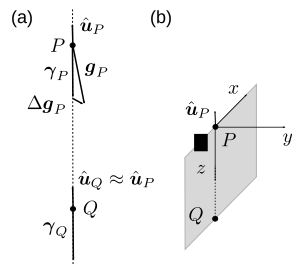
\includegraphics{figures/local-system.png}
    \caption{(a) Schematic representation of the gravity vector
    $\mitbf{g}_{P}$, normal gravity vector $\mitbf{\gamma}_{P}$,
    disturbing gravitational attraction $\Delta \mitbf{g}_{P}$
    (equation \ref{eq:gravity-vector}) and the unit vector 
    $\hat{\mitbf{u}}_{P}$ (equation \ref{eq:unit-vectors}) 
    at the point $P$ and also the normal gravity vector
    $\mitbf{\gamma}_{Q}$ at the point $Q$ on the reference ellipsoid.
    At the point $P$ the normal gravity vector $\mitbf{\gamma}_{P}$ 
    is opposite to the unit vector $\hat{\mitbf{u}}_{P}$ and the 
    normal gravity $\mitbf{\gamma}_{Q}$ at the point $Q$ is opposite
    the another unit vector $\hat{\mitbf{u}}_{Q}$, which is
    close to $\hat{\mitbf{u}}_{P}$.
    (b) Schematic representation of a topocentric Cartesian 
    coordinate system with origin at a point $P$ and $x$, $y$ and $z$ 
    axes defined by the unit vectors $\hat{\mitbf{v}}_{P}$, 
    $\hat{\mitbf{w}}_{P}$ and $-\hat{\mitbf{u}}_{P}$ 
    (Figure \ref{fig:fig1}), respectively.}
  \label{fig:fig2}
\end{figure}

\label{lastpage}


\end{document}